\documentclass[letterpaper, reqno,11pt]{article}
\usepackage[margin=1.0in]{geometry}
\usepackage{color,latexsym,amsmath,amssymb,graphicx,float,listings,tikz}
\usepackage{hyperref}

\hypersetup{
colorlinks=true,
linkcolor=magenta,
filecolor=magenta,
urlcolor=cyan,
}

\lstset{
basicstyle=\ttfamily,
columns=fullflexible,
frame=single,
breaklines=true,
postbreak=\mbox{\textcolor{red}{$\hookrightarrow$}\space},
}

\graphicspath{ {images/} }

\begin{document}
\pagenumbering{arabic}
\title{PHYS 408 Homework 4}
\date{21/03/24}
\author{Xander Naumenko}
\maketitle

{\medskip\noindent\bf Question 1a.} The propagation equation is:
\[
\vec E(\vec r)=\vec E_0 \frac{w_0}{w(z)}\text{exp}\left( \frac{\rho^2}{w^2(z)} \right) \text{exp}\left( ik \frac{\rho^2}{2R(z)} \right) \text{exp}\left( ikz-i\tan^{-1}\left( \frac{z}{z_0} \right)  \right) 
.\]
The only difference between the beams is the propagation distances $z$. We can use the formula we derived in class to get the intensity: $I=I_1+I_2+2\sqrt{I_1I_2}\cos(\Delta\phi)$:
\[
I=\frac{I_0w_0^2e^{-\frac{2\rho^2}{w^2(z_s-z_1)}}}{w(z_s-z_1)^2}+\frac{I_0w_0^2e^{-\frac{2\rho^2}{w^2(z_s-z_2)}}}{w(z_s-z_2)^2}+2\frac{I_0w_0^2e^{-\frac{\rho^2}{w^2(z_s-z_2)}-\frac{\rho^2}{w^2(z_s-z_1)}}}{w(z_s-z_2)w(z_s-z_1)}\cos\Delta\phi
.\]
$I_0$, $R(z)$, $w(z)$, etc. are all defined as we did in class. Here $\Delta\phi$ is the difference in phase between the waves, which we know from the first expression is:
\[
    \Delta\phi=\frac{k\rho^2}{2}\left( \frac{1}{R(z_s-z_1)}+\frac{1}{R(z_s-z_2)} \right)+k\left( 2z_s-z_1-z_2 \right)-\left( \tan^{-1}\left( \frac{z_s-z_1}{z_0} \right) +\tan^{-1}\left( \frac{z_s-z_2}{z_0} \right) \right) 
.\]
It might be possible to clean this up a bit, but given we're plotting it numerically next and the question doesn't ask for it this is fine. The interference pattern that this produces comes from the phase, which results in concentric circles of alternating on and off sections.

{\medskip\noindent\bf Question 1b.} See figure \ref{fig:q1} for the full 2d distribution. The code used to produce it was:

\begin{figure}[htpb]
    \centering
    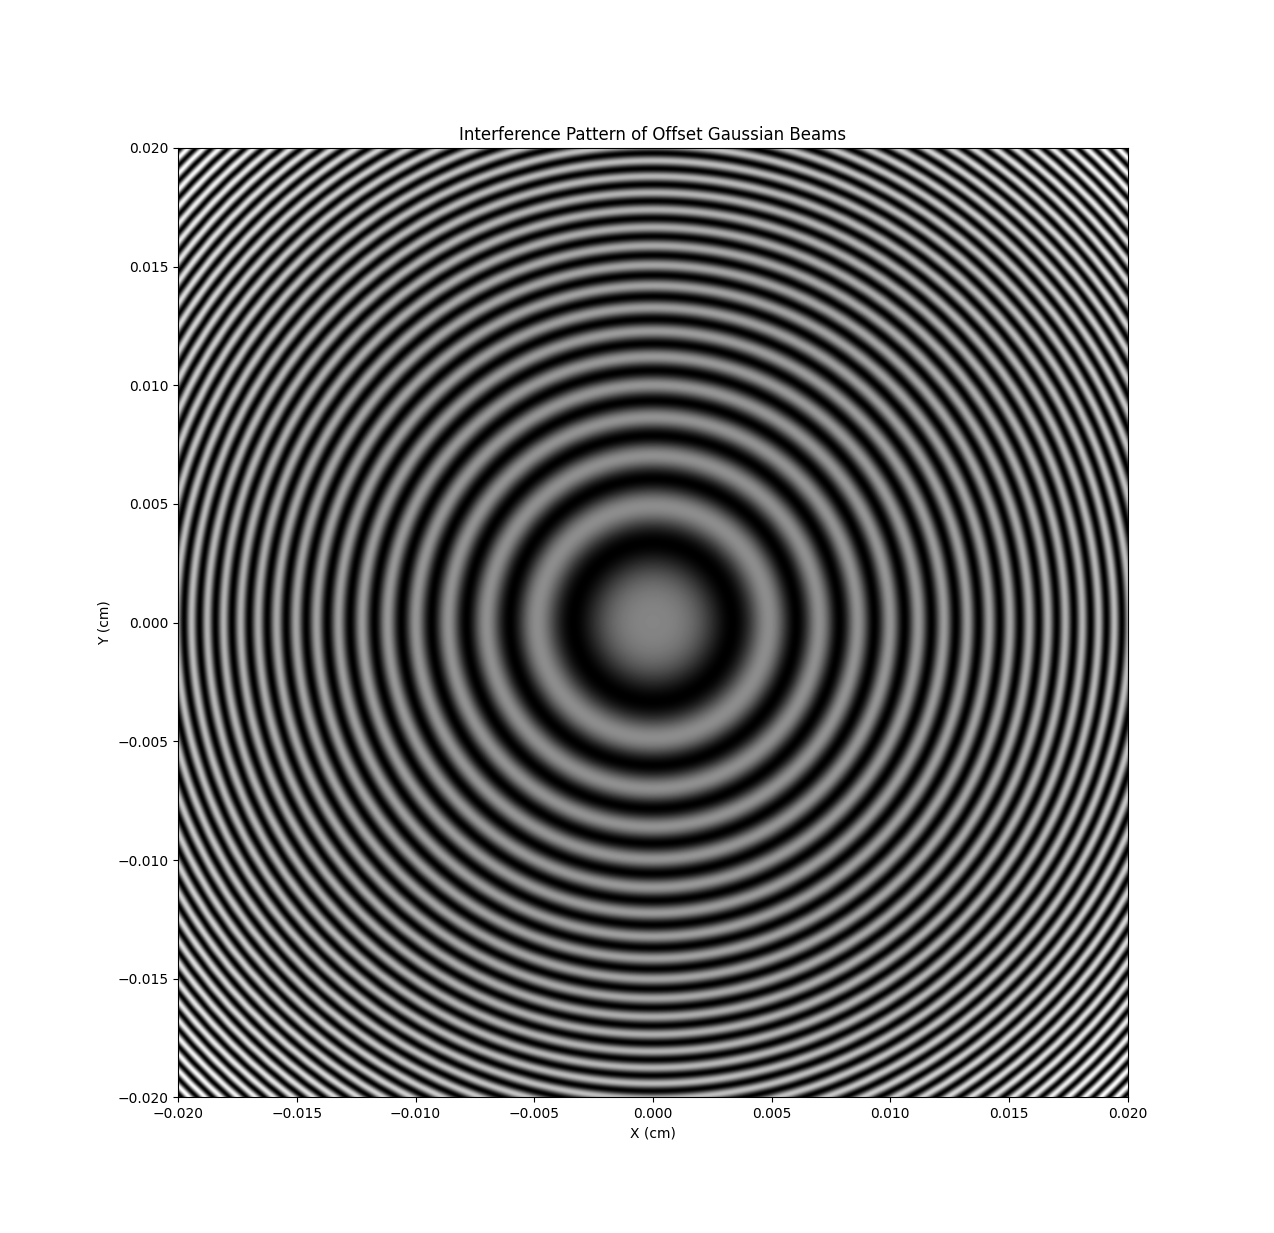
\includegraphics[width=0.8\textwidth]{q1}
    \caption{Intensity distribution for question 1b. As expected, many concentric circles of intensity are seen.}
    \label{fig:q1}
\end{figure}
\begin{lstlisting}
import matplotlib.pyplot as plt

import numpy as np

lam = 633e-9
w0 = 4e-6
d = 0.05
D = 1
scr = 0.02
N = 1000
z0 = w0**2*np.pi/lam
k = 2*np.pi/lam

x = np.linspace(-scr, scr, N, dtype=np.cdouble)
y = np.linspace(-scr, scr, N, dtype=np.cdouble)

X, Y = np.meshgrid(x, y)

I = np.zeros((N, N))

def w(z):
    return w0*np.sqrt(1+(z/z0)**2)
def R(z):
    return z*(1+(z0/z)**2)

rho = (X**2+Y**2)**0.5
E = np.zeros_like(X)
for z in (D-d/2, D+d/2):
    E += w0/w(z)*np.exp(rho**2/w(z)**2)*np.exp(1j*k*rho**2/2/R(z))*np.exp(1j*k*z-1j*np.arctan(z/z0))
I = np.abs(E)**2

plt.imshow(I, extent=(-scr, scr, -scr, scr), origin='lower', cmap='gray')
plt.xlabel('X (cm)')
plt.ylabel('Y (cm)')
plt.title('Interference Pattern of Offset Gaussian Beams')
plt.show()
\end{lstlisting}

{\medskip\noindent\bf Question 2a.} Using the equations from lecture 9 equations with $\theta_i=\theta_t=0$:
\[
r=\frac{n_i-n_t}{n_t+n_i}\implies r_{12}= \frac{n_1-n_2}{n_1+n_2}, r_{23}= \frac{n_2-n_3}{n_2+n_3}, r_{21}= \frac{n_2-n_1}{n_1+n_2}
\]
\[
t=\frac{2n_i}{n_i+n_t}\implies t_{12}=\frac{2n_1}{n_1+n_2}, t_{23}=\frac{2n_2}{n_2+n_3}, t_{21}=\frac{2n_2}{n_1+n_2}
.\]

{\medskip\noindent\bf Question 2b.} 
\[
    E_t= E_iit_{12}t_{23}\sum_{i=0}^{\infty}\left(-r_{23}r_{21} \right)^{i} 
.\]
\[
    E_r = E_i \left( r_{12}-t_{12}r_{23}t_{21}\sum_{i=0}^{\infty}\left(-r_{23}r_{21}\right)^{i} \right) 
.\]

{\medskip\noindent\bf Question 2c.} 
\[
E_t = E_ii\frac{t_{12}t_{23}}{1+r_{23}r_{21} }= E_ii\frac{4n_1n_2}{(n_1+n_2)(n_2+n_3)+(n_2-n_1)(n_2-n_3)}=E_ii \frac{4n_1n_2}{n_2^2+n_1n_3}
.\]
\[
E_r = E_i \left(\frac{n_1-n_2}{n_1+n_2}-\frac{4n_1n_2(n_2-n_3)}{(n_1+n_2)^2(n_2+n_3)}\frac{1}{1+(n_2-n_1)(n_2-n_3)/\left( (n_1+n_2)(n_2+n_3) \right) } \right)
\]
\[
= E_i \frac{n_1n_3-n_2^2}{n_2^2+n_1n_3}
.\]

{\medskip\noindent\bf Question 2d.} Setting $n_2=\sqrt{n_1n_3}$, we can easily see that the expression for reflection goes to zero:
\[
E_r=E_i \frac{0}{2n_1n_3}=0
.\]

{\medskip\noindent\bf Question 3a.} The stability criterion:
\[
0\leq g_1g_2= \left( 1+\frac{d}{R_1} \right) \left( 1+\frac{d}{R_2} \right) \leq 1
\]
\[
\implies 0\leq (d-15)(d-8)\leq 120
.\]
Thus the system is stable for $0\leq d\leq 8$ and $15\leq d\leq 23$ ($23$ being the root of $(d-15)(d-8)-120=0$), and unstable otherwise.

{\medskip\noindent\bf Question 3b.} From Steck 7.65, plugging in $d=5$ and $d=17$ respectively:
\[
z_0^2= \frac{-d(R_1+d)(R_2+d)(R_2+R_1+d)}{\left( R_2+R_1+2d \right) ^2}= 15.98 \text{ or }15.17
.\]
% \[
% z_0^2=\frac{g_1g_2(1-g_1g_2)}{(g_1+g_2-2g_1g_2)^2}d^2=15.98 \text{ or }15.17
% .\]
The $q$-parameter is then the following as a function of $z$, with $z_0$ replaced with the square root of one of the above values depending on the two possible values of $d$:
\[
q(z)=z-iz_0
.\]

{\medskip\noindent\bf Question 3c.} Plugging $d=10$ into the previous expression for $z_0^2$, it gives $z_0^2=-144.4\implies z_0\approx 12i$. This leads to an unstable mode, since if we recall back to the purpose of introducing $z_0$ was to shift $z\rightarrow z-iz_0$. This eliminated the problem of paraxial solutions to the wave equation taking up all of space which is clearly unphysical, which is what we're seeing here since $z_0\propto i$. Thus such a Gaussian wave can't exist.

{\medskip\noindent\bf Question 3d.} From Steck 7.80, we have
\[
\nu_{l,m,z}=\frac{c}{d}\left(q+\frac{1}{\pi}\left( 1+l+m \right) \cos^{-1}\sqrt{g_1g_2}\right)
.\]
Since there aren't too many values of $l,m$ that are possible we can just try all of them:
\begin{lstlisting}
import numpy as np

c = 3e8
nu = 4.74e12
d = 5
R1 = -8
R2 = -15
g1 = 1+d/R1
g2 = 1+d/R2

for lm in range(0,7):
    q = nu*d/c-1/np.pi*(1+lm)*np.arccos(np.sqrt(g1*g2))
    print(q)
\end{lstlisting}
Doing this gives that only $q=78999$ and $q=78998$ are possible.

{\medskip\noindent\bf Question 4a.} See figure \ref{fig:q4a}. The calculations confirm that the stack acts as a decent reflector, although still around $\frac{1}{7}$ of the light makes it through. To make it a better reflector, we could increase the difference between $n_1$ and $n_2$, as this would make the $M_{12}^{-1}$ and $M_{21}^{-1}$ to be larger.\begin{figure}[htpb]
    \centering
    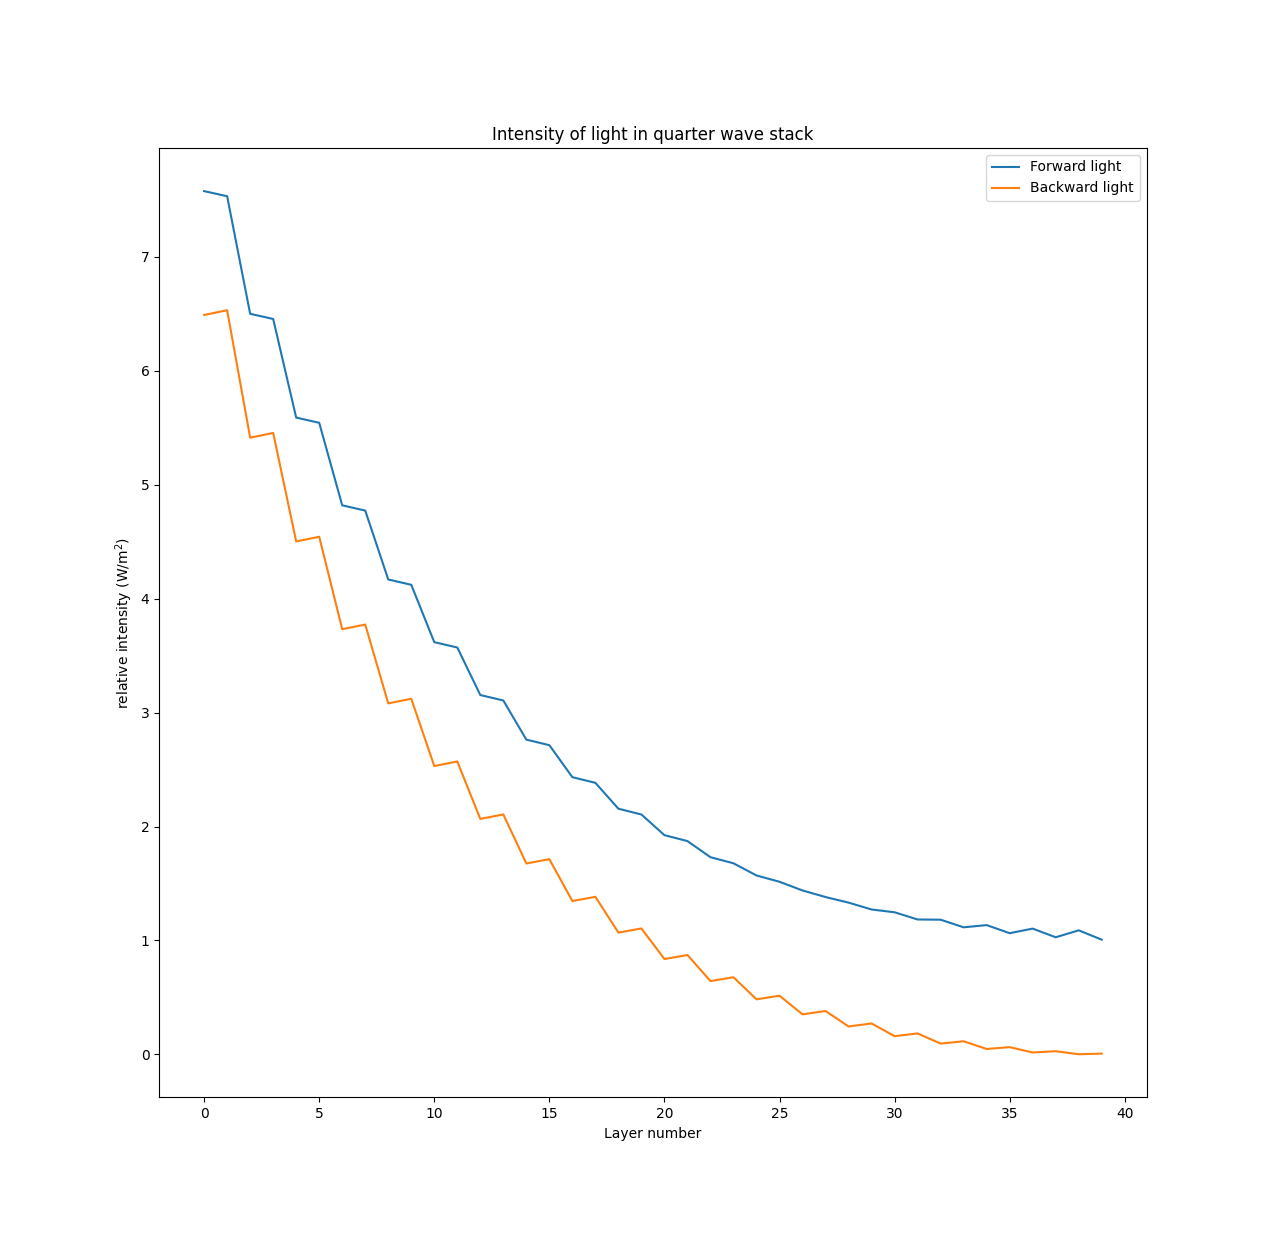
\includegraphics[width=0.8\textwidth]{q4a}
    \caption{Graph for question 4a.}
    \label{fig:q4a}
\end{figure}

{\medskip\noindent\bf Question 4b.} See figure \ref{fig:q4b}. With the addition of the impurity no light is reflected whatsoever, and it is all reflected. This is due to the defect mode, if we changed one of the layers to be even slightly off from a quarter wave then this effect would disappear and as we saw in class it would go back to reflection. This was the code used for both parts of this question:

\begin{figure}[htpb]
    \centering
    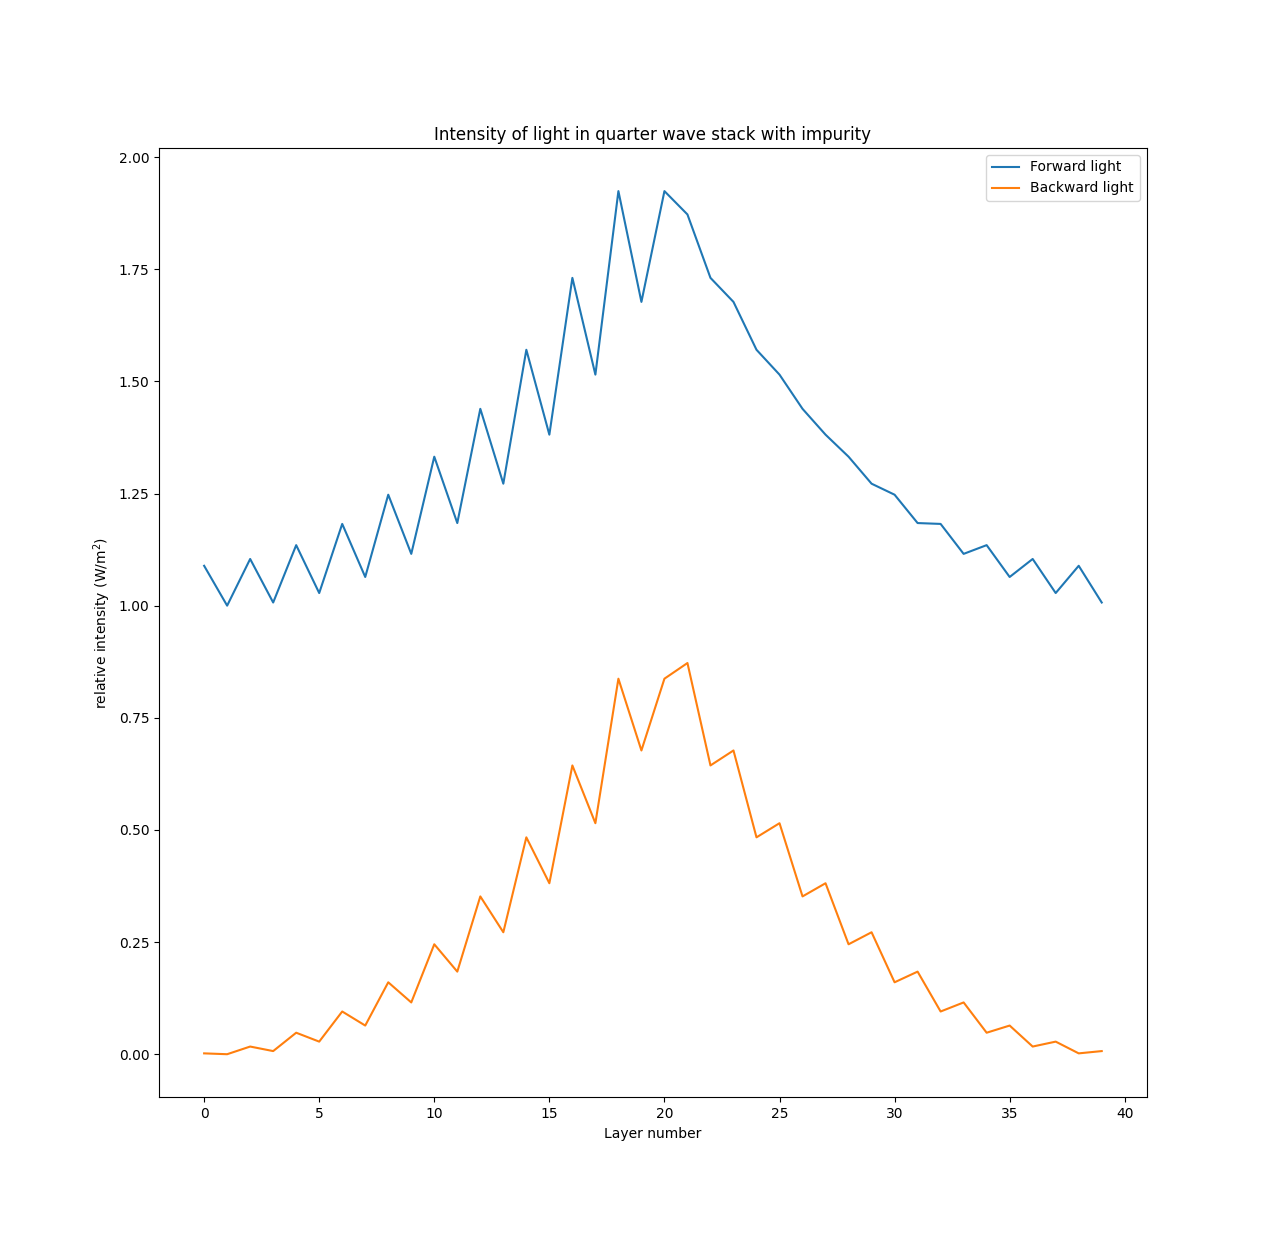
\includegraphics[width=0.8\textwidth]{q4b}
    \caption{Graph for question 4b.}
    \label{fig:q4b}
\end{figure}

\begin{lstlisting}
import numpy as np

import matplotlib.pyplot as plt

n1 = 1.5
n2 = 1.38
n3 = 1.77

M21 = 1/(2*n2)*np.array([[n2+n1, n2-n1], [n2-n1, n2+n1]])
M12 = 1/(2*n1)*np.array([[n2+n1, n1-n2], [n1-n2, n2+n1]])
M13 = 1/(2*n1)*np.array([[n3+n1, n1-n3], [n1-n3, n3+n1]])
M31 = 1/(2*n3)*np.array([[n1+n3, n3-n1], [n3-n1, n1+n3]])

Md = np.array([[1j, 0], [0, -1j]], dtype=np.cdouble)
Ms = np.array([[-1, 0], [0, -1]])

M21inv = np.linalg.inv(M21)
M12inv = np.linalg.inv(M12)
Mdinv = np.linalg.inv(Md)
Msinv = np.linalg.inv(Ms)
M13inv = np.linalg.inv(M13)
M31inv = np.linalg.inv(M31)

N = 20

U_for = np.zeros(2*N, dtype=np.cdouble)
U_back = np.zeros(2*N, dtype=np.cdouble)

U = np.array([1, 0])

for i in range(1, int(N/2+1)):
    U = np.matmul(Mdinv, U)
    U = np.matmul(M12inv, U)
    U_for[2*N-2*i] = U[0]
    U_back[2*N-2*i] = U[1]
    U = np.matmul(Mdinv, U)
    U = np.matmul(M12, U)
    U_for[2*N-2*i+1] = U[0]
    U_back[2*N-2*i+1] = U[1]

U = np.matmul(Mdinv, U)
U = np.matmul(M13, U)
U = np.matmul(Msinv, U)
U = np.matmul(M31, U)

for i in range(int(N/2+1), N+1):
    U = np.matmul(Mdinv, U)
    U = np.matmul(M12inv, U)
    U_for[2*N-2*i] = U[0]
    U_back[2*N-2*i] = U[1]
    U = np.matmul(Mdinv, U)
    U = np.matmul(M12, U)
    U_for[2*N-2*i+1] = U[0]
    U_back[2*N-2*i+1] = U[1]

print(U)
plt.plot(np.abs(U_for)**2, label='Forward light')
plt.plot(np.abs(U_back)**2, label='Backward light')
plt.legend()
plt.xlabel('Layer number')
plt.ylabel('relative intensity (W/m$^2$)')
plt.title('Intensity of light in quarter wave stack with impurity')
plt.show()

\end{lstlisting}



\end{document}
